\documentclass[11pt]{article}
\usepackage{house}
\hypersetup{pdftitle={Cointegration-Based Pairs Trading in Indian Bank Stocks: A Walk-Forward Evaluation}, pdfauthor={Arjun Prashanth}, pdfkeywords={pairs trading, statistical arbitrage, cointegration, walk-forward backtest, India}}
% Generated by paper/make_assets.py. Do not edit by hand.
\newcommand{\NUniverse}{14}
\newcommand{\NTraded}{11}
\newcommand{\NCandidates}{55}
\newcommand{\NWindows}{19}
\newcommand{\FormMonths}{12}
\newcommand{\TradeMonths}{6}
\newcommand{\EntryZ}{2}
\newcommand{\ExitZ}{0.5}
\newcommand{\StopZ}{4}
\newcommand{\MaxHold}{60}
\newcommand{\BpsLeg}{20}
\newcommand{\PThreshold}{0.05}
\newcommand{\MaxPairs}{5}
\newcommand{\SampleStart}{2016-01-01}
\newcommand{\SampleEnd}{2026-07-31}
\newcommand{\OOSStart}{2017-01-02}
\newcommand{\OOSEnd}{2026-06-30}
\newcommand{\OOSDays}{2{,}347}
\newcommand{\Capital}{100{,}000}
\newcommand{\NConvStop}{201}
\newcommand{\PairWindows}{77}
\newcommand{\UniquePairs}{45}
\newcommand{\MedianP}{0.015}
\newcommand{\MedianHalfLife}{6.8}
\newcommand{\RetG}{\ensuremath{+1.27}\%}
\newcommand{\VolG}{7.27\%}
\newcommand{\SharpeG}{\ensuremath{-0.65}}
\newcommand{\DDG}{13.59\%}
\newcommand{\GrowthG}{1.12}
\newcommand{\RetN}{\ensuremath{-1.29}\%}
\newcommand{\VolN}{7.30\%}
\newcommand{\SharpeN}{\ensuremath{-1.00}}
\newcommand{\DDN}{20.17\%}
\newcommand{\GrowthN}{0.89}
\newcommand{\RetU}{13.81\%}
\newcommand{\VolU}{25.31\%}
\newcommand{\SharpeU}{0.31}
\newcommand{\DDU}{57.95\%}
\newcommand{\GrowthU}{3.34}
\newcommand{\RetM}{12.18\%}
\newcommand{\VolM}{16.35\%}
\newcommand{\SharpeM}{0.38}
\newcommand{\DDM}{38.44\%}
\newcommand{\GrowthM}{2.92}
\newcommand{\NTrades}{242}
\newcommand{\MeanHold}{15.9}
\newcommand{\MedianHold}{11}
\newcommand{\WinGross}{52.1\%}
\newcommand{\WinNet}{46.7\%}
\newcommand{\MeanGrossPnL}{192}
\newcommand{\MeanGrossBps}{19}
\newcommand{\MeanCost}{403}
\newcommand{\MeanCostBps}{40}
\newcommand{\MeanDailyBps}{0.61}
\newcommand{\NWtGross}{0.67}
\newcommand{\NWpGross}{0.50}
\newcommand{\NWtNet}{\ensuremath{-0.46}}
\newcommand{\NWpNet}{0.65}
\newcommand{\TradeT}{0.70}
\newcommand{\NConv}{71}
\newcommand{\NStop}{130}
\newcommand{\NTimeout}{8}
\newcommand{\NWindowEnd}{33}
\newcommand{\ShareStop}{53.7\%}
\newcommand{\ShareStopRound}{54\%}
\newcommand{\StopToConv}{1.8}
\newcommand{\ConvGross}{320{,}605}
\newcommand{\StopGross}{305{,}070}
\newcommand{\AvgConv}{4{,}516}
\newcommand{\AvgStop}{2{,}347}
\newcommand{\BreakEvenMix}{34.2\%}
\newcommand{\RealisedMix}{35.3\%}
\newcommand{\BinomMixP}{0.77}
\newcommand{\StopMedianHold}{3.5}
\newcommand{\StopWithinFour}{68}
\newcommand{\ConvMedianHold}{14}
\newcommand{\ConvHalfLife}{6.4}
\newcommand{\ConvRatio}{1.98}
\newcommand{\ConvEntryZ}{2.27}
\newcommand{\ConvDecay}{4.5}
\newcommand{\ConvHalfLives}{2.2}
\newcommand{\ChiTwo}{3.40}
\newcommand{\ChiDof}{2}
\newcommand{\ChiP}{0.18}
\newcommand{\NFullYears}{9}
\newcommand{\NYearsPos}{6}
\newcommand{\NWindowsPos}{12}
\newcommand{\GrossTwentyTwenty}{\ensuremath{-9.86}\%}
\newcommand{\WorstWindowLoss}{43{,}737}
\newcommand{\TotalGross}{46{,}368}
\newcommand{\WorstWindowStart}{2025-01-01}
\newcommand{\NConcentrated}{7}
\newcommand{\KotakSameDay}{4}
\newcommand{\KotakPairsSelected}{4}
\newcommand{\KotakEntry}{2025-01-21}
\newcommand{\KotakExit}{2025-03-24}
\newcommand{\KotakEach}{12{,}500}
\newcommand{\KotakFedExit}{2025-03-20}
\newcommand{\KotakFedLoss}{7{,}236}
\newcommand{\KotakSameDayLoss}{44{,}660}
\newcommand{\AxisFedStops}{6}
\newcommand{\AxisFedLoss}{20{,}810}
\newcommand{\IndIdfcTrades}{7}
\newcommand{\IndIdfcLoss}{20{,}500}
\newcommand{\BreakEven}{9.8}
\newcommand{\BreakEvenSimple}{9.6}
\newcommand{\Beta}{\ensuremath{-0.026}}
\newcommand{\BetaMove}{0.03}
\newcommand{\CorrMkt}{\ensuremath{-0.057}}
\newcommand{\RsqMkt}{0.3}
\newcommand{\ExP}{0.017}
\newcommand{\ExHalfLife}{6.4}
\newcommand{\ExTimesSelected}{4}
\newcommand{\OldTrades}{1{,}008}
\newcommand{\OldBeyondStop}{816}
\newcommand{\OldStops}{892}
\newcommand{\OldNet}{\ensuremath{-9.82}\%}
\newcommand{\OldGross}{\ensuremath{+1.04}\%}
\newcommand{\FixNetChange}{8.5}
\newcommand{\FixGrossChange}{0.2}
\newcommand{\OldBreakEven}{1.9}


\title{Cointegration-Based Pairs Trading in Indian Bank Stocks\\[0.25em]
  \large\mdseries A Walk-Forward Evaluation}
\shorttitle{Pairs trading in Indian bank stocks}
\author{Arjun Prashanth\thanks{Email: \href{mailto:arjunprashanth6129@gmail.com}{arjunprashanth6129@gmail.com}.
  Code, tests, results and the script that generates every number, table and
  figure in this paper are at
  \weburl{https://github.com/arjunprashanth6129/}{pairs-trading-backtester}. An
  interactive summary of the results is at
  \weburl{https://arjun-quant-projects.vercel.app/}{pairs-trading}.}}
\date{October 2026}
\keywords{pairs trading; statistical arbitrage; cointegration; walk-forward
  backtest; transaction costs; market neutrality; Indian banks}
\jel{C32, G11, G14, G17}

\begin{document}
\maketitle
\thispagestyle{plain}

\begin{abstract}
I evaluate a cointegration-based pairs-trading strategy on \NTraded{} banks listed
on India's National Stock Exchange. Every six months from January 2017 to June
2026, all \NCandidates{} pairs are tested with the Engle-Granger procedure on the
preceding twelve months, and up to five cointegrated pairs are traded over the
next six months on a fixed z-score rule. Every parameter is estimated before
trading begins, and costs of \BpsLeg{} basis points are charged on each leg. Over
\OOSDays{} out-of-sample days and \NTrades{} round trips, the strategy returns
\RetG{} a year before costs and \RetN{} after, and the gross return is not
distinguishable from zero (Newey-West $t = \NWtGross$). It is market-neutral,
with a beta of \Beta{} to the Nifty 50. Its weakness is persistence: \ShareStopRound{}
of trades are stopped out, more than converge, and the formation-period $p$-value
does not predict which. The break-even cost is \BreakEven{} basis points per leg.
\end{abstract}

% ======================================================================
\section{Introduction}

Pairs trading takes offsetting positions in two securities whose prices have
historically moved together. When their relationship diverges, the strategy buys
the relatively cheap security and sells the relatively expensive one, and it closes
the position when the relationship reverts. Because the two legs offset, the
position is designed to be insensitive to the direction of the market.
\citet{gatev2006} report average annualised excess returns of up to 11\% for a
version of the rule that matches US stocks by the distance between their
normalised prices from 1962 to 2002. \citet{do2010} find that the profitability of
the same rule declined substantially in later years, and \citet{krauss2017} reviews
the main variants that have since been proposed.

The variant studied here selects pairs by cointegration \citep{engle1987}, a
stricter condition than correlation. Two prices can have highly correlated daily
returns and still drift apart without limit if one has a slightly higher trend. If
instead some linear combination $y_t - \beta x_t$ is stationary, deviations from its
mean are expected to decay, which is the property a convergence trade depends on
\citep{vidyamurthy2004}. \citet{avellaneda2010} apply the same idea of trading
mean-reverting residuals at the scale of the US equity market.

This paper asks whether that property survives out of sample in a setting where it
is economically plausible: if pairs of Indian bank stocks are selected by a
cointegration test on twelve months of prices and traded on a fixed rule over the
following six months, does the strategy earn a positive return after costs, and is
that return independent of the market? Banks share a regulator, an interest-rate
cycle and a credit cycle, so a stable long-run relationship between their prices
has an economic basis. Every parameter is estimated on data that precede the
period in which it is used, and the code that enforces this is covered by tests
that fail if the separation is broken.

The strategy works as a hedge and fails as a source of return. Its beta to the
Nifty 50 is close to zero, but its return before costs, \RetG{} a year, is not
statistically different from zero and is below the risk-free rate. A decomposition
of the \NTrades{} trades explains why. Trades that converged did so, on average, at
the speed the formation period predicted, but \NStop{} of the \NTrades{} were
stopped out after the spread widened further, and the losses on those trades
cancelled the gains on the rest. The formation $p$-value carries no information
about which pairs will hold. The largest single loss came from four simultaneous
positions that were in effect one bet on a single bank.

The paper contributes a careful out-of-sample test of the cointegration approach in
an emerging-market sector, a decomposition by exit type that identifies the
mechanism behind the null result, and a record of an implementation error found
during validation and how it changed the results (Appendix~\ref{app:fix}).
Section~\ref{sec:data} describes the data and Section~\ref{sec:method} the method.
Section~\ref{sec:results} presents the results, Section~\ref{sec:discussion}
discusses them and Section~\ref{sec:limits} sets out their limitations.
Section~\ref{sec:conclusion} concludes.

% ======================================================================
\section{Data}\label{sec:data}

The universe is \NUniverse{} banks listed on the National Stock Exchange. Daily
closing prices adjusted for splits and dividends were downloaded from Yahoo
Finance for \SampleStart{} to \SampleEnd. Three banks, RBL Bank (listed August
2016), AU Small Finance Bank (July 2017) and Bandhan Bank (March 2018), have price
histories covering less than 95\% of the sample and are excluded. The remaining
\NTraded{} are HDFC Bank, ICICI Bank, Axis Bank, Kotak Mahindra Bank, State Bank of
India, IndusInd Bank, Federal Bank, Bank of Baroda, Punjab National Bank, Canara
Bank and IDFC First Bank, giving $\binom{11}{2} = \NCandidates$ candidate pairs. Only
dates on which all \NTraded{} traded are retained. The out-of-sample period runs
from \OOSStart{} to \OOSEnd, \OOSDays{} trading days. The Nifty 50 index is used only
to measure market exposure, and the risk-free rate is 6\% a year.

% ======================================================================
\section{Method}\label{sec:method}

\subsection{Formation and trading periods}

The sample is divided into \NWindows{} windows, each a \FormMonths-month formation
period followed by a \TradeMonths-month trading period (Figure~\ref{fig:windows}).
Windows advance by six months, so the trading periods are contiguous, do not
overlap, and together cover January 2017 to June 2026. Pairs are selected and every
parameter is estimated in the formation period, and they are then held fixed for
the whole trading period.

\begin{figure}[tbp]
\centering
\begin{tikzpicture}[x=1.45cm,y=0.58cm]
  % One unit is one year from January 2016.
  \draw[rule, line width=0.6pt] (0,0) -- (10.75,0);
  \foreach \yr in {0,2,4,6,8,10}{
    \pgfmathtruncatemacro{\lab}{2016+\yr}
    \draw[rule] (\yr,0) -- (\yr,-0.18); \node[font=\scriptsize, below] at (\yr,-0.18) {\lab};}
  \foreach \k/\y in {0/3.6, 1/2.8, 2/2.0}{
    \pgfmathsetmacro{\s}{\k*0.5}
    \fill[accent!22] (\s,\y-0.28) rectangle (\s+1,\y+0.28);
    \draw[rule, line width=0.4pt] (\s,\y-0.28) rectangle (\s+1,\y+0.28);
    \fill[accentorange!60] (\s+1,\y-0.28) rectangle (\s+1.5,\y+0.28);
    \draw[rule, line width=0.4pt] (\s+1,\y-0.28) rectangle (\s+1.5,\y+0.28);
    \pgfmathtruncatemacro{\kk}{\k+1}
    \node[font=\scriptsize, anchor=west] at (\s+1.56,\y) {window \kk};
  }
  \node[font=\footnotesize] at (3.4,1.3) {$\vdots$};
  \fill[accent!22] (9,0.75-0.28) rectangle (10,0.75+0.28);
  \draw[rule, line width=0.4pt] (9,0.75-0.28) rectangle (10,0.75+0.28);
  \fill[accentorange!60] (10,0.75-0.28) rectangle (10.5,0.75+0.28);
  \draw[rule, line width=0.4pt] (10,0.75-0.28) rectangle (10.5,0.75+0.28);
  \node[font=\scriptsize, anchor=east] at (8.94,0.75) {window \NWindows};
  \fill[accent!22] (5.2,4.32) rectangle (5.52,4.58); \draw[rule,line width=0.4pt] (5.2,4.32) rectangle (5.52,4.58);
  \node[font=\scriptsize, anchor=west] at (5.56,4.45) {formation, 12 months: test, select, estimate $\beta$, $\mu_s$, $\sigma_s$, $h$};
  \fill[accentorange!60] (5.2,3.82) rectangle (5.52,4.08); \draw[rule,line width=0.4pt] (5.2,3.82) rectangle (5.52,4.08);
  \node[font=\scriptsize, anchor=west] at (5.56,3.95) {trading, 6 months: apply the rule, parameters fixed};
  \draw[decorate, decoration={brace, amplitude=4pt, mirror}, rule]
    (1,-0.95) -- (10.5,-0.95) node[midway, below=4pt, font=\scriptsize]
    {out-of-sample trading periods, \OOSStart{} to \OOSEnd};
\end{tikzpicture}
\caption{Formation and trading periods, drawn to scale. Each window's twelve-month
formation period (blue) selects the pairs and fixes their parameters; the following
six-month trading period (orange) applies them without re-estimation. Windows
advance by six months, so trading periods tile the out-of-sample period. Only the
first three and the last of the \NWindows{} windows are shown.}
\label{fig:windows}
\end{figure}

\subsection{Pair selection}

In each formation period, every candidate pair is tested with the two-step
procedure of \citet{engle1987}. The first step estimates the hedge ratio by
ordinary least squares,
\begin{equation}\label{eq:hedge}
  y_t = \alpha + \beta x_t + e_t ,
\end{equation}
and the second tests the residual $e_t$ for a unit root with an augmented
Dickey-Fuller test \citep{dickey1979}, with the lag length chosen by the Akaike
information criterion and $p$-values from the response surfaces of
\citet{mackinnon2010}, as implemented in statsmodels \citep{seabold2010}. The null
hypothesis is no cointegration. The dependent leg $y$ is the stock with the higher
average price, so that the orientation of each pair is fixed by rule rather than
chosen. Pairs with $p \le \PThreshold$ are retained, at most \MaxPairs{} per window
and lowest $p$-value first.

For each retained pair the formation period also fixes the spread mean $\mu_s$, the
spread standard deviation $\sigma_s$ and the half-life of mean reversion. The
half-life comes from a discrete approximation to an Ornstein-Uhlenbeck process,
\begin{equation}\label{eq:halflife}
  \Delta s_t = a + \kappa\, s_{t-1} + u_t, \qquad h = -\frac{\ln 2}{\kappa},
\end{equation}
estimated on the formation spread. Across the sample, \PairWindows{} pair-windows
were selected from \UniquePairs{} distinct pairs of banks, with a median $p$-value of
\MedianP{} and a median half-life of \MedianHalfLife{} trading days.

\subsection{Trading rule}

In the trading period the spread is $s_t = y_t - \beta x_t$ and its standardised
value is
\begin{equation}\label{eq:z}
  z_t = \frac{s_t - \mu_s}{\sigma_s},
\end{equation}
with $\beta$, $\mu_s$ and $\sigma_s$ taken from the formation period throughout.
Figure~\ref{fig:rule} sets out the rule. When $z_t$ rises above $+\EntryZ$ the
strategy sells the spread (sells $y$ and buys $\beta$ units of $x$), and when it falls
below $-\EntryZ$ it buys the spread. A position is closed when $|z_t|$ returns within
\ExitZ{} (converged), when $|z_t|$ reaches \StopZ{} (stopped out), after \MaxHold{}
trading days (timed out) or at the end of the trading period. No position is opened
while $|z_t| \ge \StopZ$, and at most one position per pair is open at a time.
Signals are computed from the close of day $t$ and executed at the close of day
$t+1$. The thresholds are conventional values fixed before the backtest was run;
they were not chosen by performance, which would introduce look-ahead at the level
of the parameters.

\begin{figure}[tbp]
\centering
\begin{tikzpicture}[
    st/.style={draw=rule, line width=0.5pt, rounded corners=2pt, fill=boxfill,
               align=center, font=\footnotesize, minimum width=3.0cm, minimum height=1.0cm},
    lab/.style={font=\scriptsize, align=center}]
  \node[st] (flat) at (0,0) {Flat\\ \scriptsize no position in the pair};
  \node[st] (short) at (-4.4,-1.9) {Short the spread\\ \scriptsize sell $y$, buy $\beta$ units of $x$};
  \node[st] (long) at (4.4,-1.9) {Long the spread\\ \scriptsize buy $y$, sell $\beta$ units of $x$};
  \node[st, minimum width=11.4cm, minimum height=1.15cm] (exit) at (0,-3.95)
    {Close the position when any of these holds first\\[1pt]
     \scriptsize $|z_t| \le \ExitZ$ converged \quad $|z_t| \ge \StopZ$ stopped out \quad
     \MaxHold{} days timed out \quad trading period ends};
  \draw[flow] (flat.west) -| node[lab, above, pos=0.25] {$+\EntryZ < z_t < +\StopZ$} (short.north);
  \draw[flow] (flat.east) -| node[lab, above, pos=0.25] {$-\StopZ < z_t < -\EntryZ$} (long.north);
  \draw[flow] (short.south) -- (short.south |- exit.north);
  \draw[flow] (long.south) -- (long.south |- exit.north);
  \draw[flow] (exit.north) -- node[lab, right] {back to flat} (flat.south);
\end{tikzpicture}
\caption{The trading rule. The z-score is computed from the close of day $t$ using
formation-period parameters, and every transition is executed at the close of day
$t+1$. Entry requires $|z_t|$ to lie between the entry and stop levels, so no
position is opened while the spread is already beyond the stop. At most one
position per pair is open at a time.}
\label{fig:rule}
\end{figure}

\subsection{Position sizing and costs}

Each position has a gross notional of \rupee\Capital{} (one lakh), the sum of the absolute values
of the two legs. Capital is divided equally among the pairs selected for a window,
and a pair without an open position contributes a zero return for the day. Costs
are \BpsLeg{} basis points per leg on traded notional, made up of about 5 basis
points of brokerage and taxes, 10 of half the bid-ask spread and 5 of slippage. Both
legs are charged at entry and again at exit, so a round trip costs 40 basis points
of gross notional, about \rupee 400.

\subsection{Controls against look-ahead}

A backtest that uses future information does not fail visibly; it reports better
numbers. Three mechanisms keep trading-period data out of every decision. First,
the hedge ratio, spread mean and spread standard deviation are computed by a single
function that receives only formation data. Second, the standardisation in
equation~\eqref{eq:z} takes $\mu_s$ and $\sigma_s$ as arguments rather than
computing them from its input, so a trading-period spread cannot be standardised
against its own statistics. Third, execution lags the signal by one day, because a
fill at the close that produced the signal would assume knowledge of that close
before it existed. Each mechanism is covered by unit tests, which perturb
trading-period prices and check that the fitted parameters do not change, among
other things; all 31 tests in the repository pass.

% ======================================================================
\section{Results}\label{sec:results}

\subsection{Performance}

Table~\ref{tab:performance} reports the strategy before and after costs alongside
two long-only references measured over the same days. Over the out-of-sample
period the strategy returns \RetG{} a year before costs and \RetN{} after, with
annualised volatility of about 7.3\%. The \NTrades{} round trips have a mean holding
period of \MeanHold{} trading days (median \MedianHold), and \WinGross{} are
profitable before costs and \WinNet{} after. The mean trade earns \rupee\MeanGrossPnL{}
before costs, \MeanGrossBps{} basis points of its notional, and pays
\rupee\MeanCost, or \MeanCostBps{} basis points.

\begin{table}[tbp]
\centering
\caption{Out-of-sample performance}
\label{tab:performance}
\small
\begin{tabular}{@{}lrrrr@{}}
\toprule
 & \multicolumn{2}{c}{Pairs strategy} & \multicolumn{2}{c}{Long-only references} \\
\cmidrule(lr){2-3}\cmidrule(l){4-5}
 & Before costs & After costs & 11 banks, equal weight & Nifty 50 \\
\midrule
Growth of 1 & 1.12 & 0.89 & 3.34 & 2.92 \\
Annualised return (\%) & $+$1.27 & $-$1.29 & $+$13.81 & $+$12.18 \\
Annualised volatility (\%) & 7.27 & 7.30 & 25.31 & 16.35 \\
Sharpe ratio, $r_f = 6\%$ & $-$0.65 & $-$1.00 & $+$0.31 & $+$0.38 \\
Maximum drawdown (\%) & 13.59 & 20.17 & 57.95 & 38.44 \\
\bottomrule
\end{tabular}

\begin{tablenote}
\OOSStart{} to \OOSEnd, \OOSDays{} trading days. The pairs strategy is reported
before and after costs of \BpsLeg{} basis points per leg. The equal-weight reference
holds the \NTraded{} traded banks; the Nifty 50 reference holds the index. Returns
are compound annual returns.
\end{tablenote}
\end{table}

The gross return is not distinguishable from zero. The mean daily return before
costs is \MeanDailyBps{} basis points, and with Newey-West standard errors
\citep{newey1987} with ten lags its $t$-statistic is \NWtGross{} ($p = \NWpGross$);
after costs it is \NWtNet{} ($p = \NWpNet$). At the trade level, the mean gross
profit has a $t$-statistic of \TradeT. The Sharpe ratio is negative even before
costs, \SharpeG, because the gross return is below the 6\% risk-free rate. A
market-neutral portfolio would in practice earn interest on the collateral it
posts, which this backtest does not credit (Section~\ref{sec:limits}).

\begin{figure}[tbp]
\centering
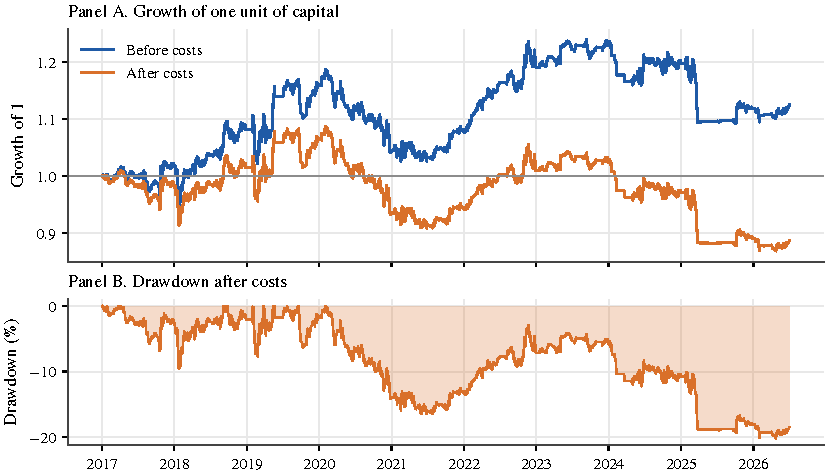
\includegraphics[width=\textwidth]{figures/equity.pdf}
\caption{Out-of-sample growth of one unit of capital before and after costs
(Panel A), and the drawdown of the after-cost series from its running peak
(Panel B). The gap between the two series in Panel A is the cumulative cost of
\NTrades{} round trips.}
\label{fig:equity}
\end{figure}

Figure~\ref{fig:equity} shows the path. The before-cost series rises to about 1.24
in September 2023 and then gives back about half of its gain, most of it in March
2025. That episode and an earlier decline in 2020 are examined in
Section~\ref{sec:periods}. The
after-cost series has the same shape and ends \GrowthN{} against \GrowthG.

\subsection{An example pair}

Figure~\ref{fig:example} shows HDFC Bank against Kotak Mahindra Bank in the first
trading window. The pair passed the formation test with $p = \ExP$ and a half-life
of \ExHalfLife{} days, and it is one of \NTopPairs{} pairs selected in
\ExTimesSelected{} windows, more often than any other. The window contains every outcome the rule
can produce. The first position opened just above $+2$, kept widening and was
stopped out in late February. Three short positions, opened between late February
and late April, each closed when the spread returned near zero. The last, opened in
late May, was stopped out on the final day of the window as the spread rose above
$+4$ again.

\begin{figure}[tbp]
\centering
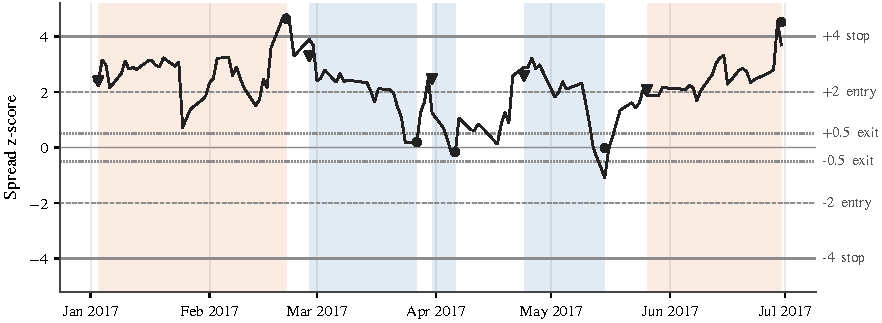
\includegraphics[width=\textwidth]{figures/example.pdf}
\caption{HDFC Bank against Kotak Mahindra Bank, January to June 2017. The line is the
spread's z-score computed with formation-period parameters. Shaded spans are
positions, blue for those closed at a profit after costs and orange for those
closed at a loss; triangles mark entries and circles exits. Markers are plotted at
execution, one day after the signal, so some entries fall inside the entry band.}
\label{fig:example}
\end{figure}

\subsection{Decomposition by exit type}

Table~\ref{tab:exits} divides the \NTrades{} trades by how they closed. The \NConv{}
trades that converged earned \rupee\ConvGross{} before costs. The \NStop{} that were
stopped out lost \rupee\StopGross. The other two exits are small. Stopped trades
therefore outnumbered converged trades by \StopToConv{} to one, and their losses
almost exactly cancelled the gains (Figure~\ref{fig:exits}, Panel A). Costs then
turned a small gross profit into a loss.

\begin{table}[tbp]
\centering
\caption{Trades by exit type}
\label{tab:exits}
\small
\begin{tabular}{@{}lrrrrrr@{}}
\toprule
Exit & Trades & Share (\%) & Gross P\&L & Costs & Net P\&L & Median days held \\
\midrule
Converged ($|z| \le 0.5$) & 71 & 29.3 & 320,605 & 28,477 & 292,128 & 14 \\
Stopped out ($|z| \ge 4$) & 130 & 53.7 & \ensuremath{-}305,070 & 52,401 & \ensuremath{-}357,471 & 3.5 \\
Timed out (60 days) & 8 & 3.3 & 10,173 & 3,243 & 6,930 & 60 \\
Trading period ended & 33 & 13.6 & 20,660 & 13,365 & 7,295 & 25 \\
\midrule Total & 242 & 100.0 & 46,368 & 97,486 & \ensuremath{-}51,118 & 11 \\
\bottomrule
\end{tabular}

\begin{tablenote}
Profit and loss in rupees, summed over all trades in each row, for positions with a
gross notional of \rupee\Capital. Costs are \BpsLeg{} basis points per leg, charged
on both legs at entry and exit.
\end{tablenote}
\end{table}

The averages make the arithmetic explicit. A converged trade earned \rupee\AvgConv{}
on average and a stopped trade lost \rupee\AvgStop. At those payoffs, converged
trades must make up at least \BreakEvenMix{} of converged and stopped trades combined
for the strategy to break even before costs. The realised share is \RealisedMix{}
(\NConv{} of the \NConvStop{} converged or stopped trades), which is not significantly different from that
threshold in a binomial test ($p = \BinomMixP$). That is why the gross return is
close to zero. A stop at $|z| = \StopZ$ means the spread moved a further two
formation standard deviations against the position, and \StopWithinFour{} of the
\NStop{} stopped trades reached that level within four trading days of entry. The
median stopped trade lasted \StopMedianHold{} days, against \ConvMedianHold{} for a
converged trade (Figure~\ref{fig:exits}, Panel B). For more than half of all trades,
a relationship that passed a cointegration test over the previous twelve months did
not hold over the following weeks.

\begin{figure}[tbp]
\centering
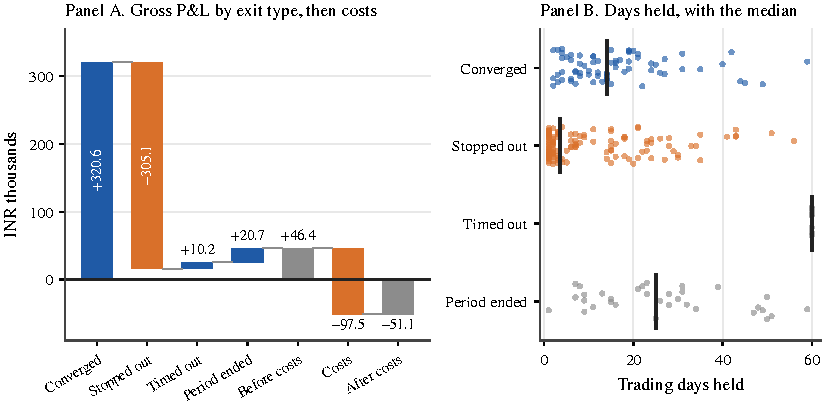
\includegraphics[width=\textwidth]{figures/exits.pdf}
\caption{Trades by exit type. Panel A builds the gross profit and loss from the four
exit types, in thousands of rupees, then deducts costs. Panel B shows how many
trading days each trade was held, one point per trade, with the median of each exit
type as a vertical bar. Trades that time out are all held for \MaxHold{} days.}
\label{fig:exits}
\end{figure}

\subsection{Speed of convergence}

The formation half-life predicts how fast a deviation should decay. For the \NConv{}
converged trades, the median holding period is \ConvMedianHold{} trading days and the
median formation half-life of the corresponding pairs is \ConvHalfLife{} days, a
ratio of \ConvRatio. That ratio is close to its theoretical value. The median
converged trade entered at $|z| = \ConvEntryZ$ and exited at \ExitZ, so the deviation
had to shrink by a factor of \ConvDecay, which takes $\log_2 \ConvDecay \approx
\ConvHalfLives$ half-lives under an autoregressive process.

Figure~\ref{fig:formation}, Panel A, makes the comparison trade by trade. It plots
each converged trade's holding period against the period predicted by its formation
half-life $h$ and entry level, $h \log_2(|z_{\mathrm{entry}}|/\ExitZ)$. The median
ratio of realised to predicted is \ConvPredRatio, so the half-life gets the typical
speed about right, but it says little about individual trades: realised holding
periods run from \ConvHoldMin{} to \ConvHoldMax{} days, and their correlation with
the prediction is \ConvPredCorr. On average, then, the estimate of speed held out of
sample. The assumption that the spread would keep reverting did not hold for most
trades.

\begin{figure}[tbp]
\centering
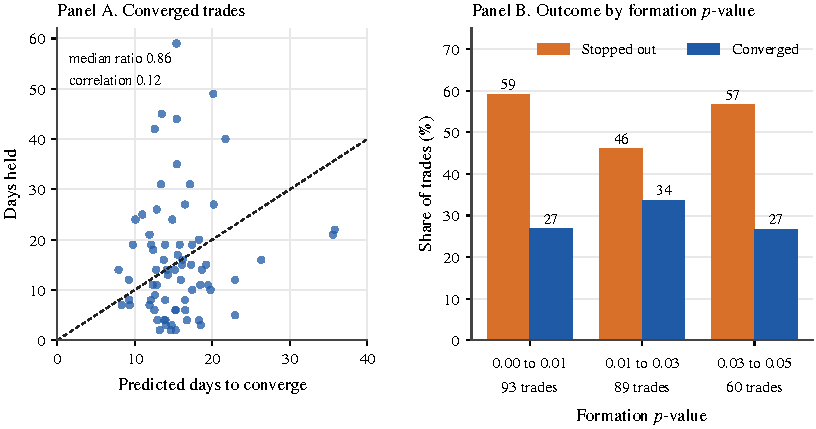
\includegraphics[width=\textwidth]{figures/formation.pdf}
\caption{What the formation period predicts. Panel A plots each of the \NConv{}
converged trades' holding period against the period predicted by its formation
half-life and entry z-score; the dashed line marks equality. Panel B shows the share
of trades stopped out and converged in each group of formation $p$-values; the
remaining trades timed out or were open at the end of the trading period.}
\label{fig:formation}
\end{figure}

\subsection{Formation \texorpdfstring{$p$}{p}-value and trade outcome}

If the formation $p$-value measured how reliable a pair's relationship would be, a
smaller $p$-value should come with fewer stop-outs. Table~\ref{tab:pvalue} and
Figure~\ref{fig:formation}, Panel B, show that it does not: the group with the
smallest $p$-values has the highest stop-out rate. A
$\chi^2$ test of independence between the $p$-value group and stopping out gives
$\chi^2(\ChiDof) = \ChiTwo$ with $p = \ChiP$. Among pairs that pass the 5\% threshold,
the $p$-value carries no detectable information about outcomes in the following six
months, so ranking pairs by it adds nothing beyond the threshold itself.

\begin{table}[tbp]
\centering
\caption{Trade outcomes by formation-period \texorpdfstring{$p$}{p}-value}
\label{tab:pvalue}
\small
\begin{tabular}{@{}lrrrr@{}}
\toprule
Formation $p$-value & Trades & Stopped out (\%) & Converged (\%) & Mean gross P\&L \\
\midrule
0.00 to 0.01 & 93 & 59.1 & 26.9 & 85 \\
0.01 to 0.03 & 89 & 46.1 & 33.7 & 302 \\
0.03 to 0.05 & 60 & 56.7 & 26.7 & 192 \\
\bottomrule
\end{tabular}

\begin{tablenote}
Trades grouped by the Engle-Granger $p$-value of their pair in the formation period.
Mean gross profit and loss per trade is in rupees.
\end{tablenote}
\end{table}

Repeated selection is no better a guide. A pair chosen in several windows has passed
the test on several different years of prices, which might be expected to signal a
durable relationship. Table~\ref{tab:toppairs} lists the \NRepeat{} pairs selected
in three or more windows. Of these, \NRepeatLoss{} lost money before costs, and
\RepeatStopShare{} of their trades were stopped out, against \ShareStop{} for all
trades.

\begin{table}[tbp]
\centering
\caption{Pairs selected in three or more windows}
\label{tab:toppairs}
\footnotesize
\setlength{\tabcolsep}{4.5pt}
\begin{tabular}{@{}lrrrrrrr@{}}
\toprule
 & & \multicolumn{2}{c}{Formation, median} & \multicolumn{3}{c}{Trades} & \\
\cmidrule(lr){3-4}\cmidrule(lr){5-7}
Pair & Windows & $p$-value & Half-life & All & Converged & Stopped & Gross P\&L \\
\midrule
HDFC Bank / Kotak Mahindra Bank & 4 & 0.018 & 6.7 & 18 & 8 & 6 & 23{,}297 \\
Canara Bank / Punjab National Bank & 4 & 0.013 & 9.9 & 9 & 3 & 3 & 4{,}861 \\
Bank of Baroda / Federal Bank & 4 & 0.002 & 6.2 & 13 & 4 & 8 & \ensuremath{-}722 \\
IDFC First Bank / IndusInd Bank & 4 & 0.003 & 5.4 & 13 & 1 & 9 & \ensuremath{-}22{,}589 \\
HDFC Bank / IndusInd Bank & 3 & 0.019 & 5.0 & 11 & 7 & 3 & 28{,}796 \\
HDFC Bank / ICICI Bank & 3 & 0.010 & 7.8 & 9 & 1 & 7 & \ensuremath{-}3{,}400 \\
ICICI Bank / State Bank of India & 3 & 0.009 & 7.8 & 6 & 1 & 5 & \ensuremath{-}4{,}605 \\
\bottomrule
\end{tabular}

\begin{tablenote}
A pair is identified by its two banks; which bank is the dependent leg can differ
between windows. The $p$-value and half-life (in trading days) are medians over the
windows in which the pair was selected. Gross profit and loss is summed over the
pair's trades, in rupees, before costs.
\end{tablenote}
\end{table}

\subsection{Performance by period and concentration}\label{sec:periods}

Before costs the strategy was profitable in \NYearsPos{} of \NFullYears{} full calendar
years and in \NWindowsPos{} of \NWindows{} trading windows (Figure~\ref{fig:years},
Panel A). The losses are concentrated in a few episodes. In 2020 the strategy lost
\GrossTwentyTwenty{} before costs. During the COVID-19 sell-off bank stocks fell by
very different amounts, and two pairs account for most of the loss: Axis Bank
against Federal Bank was stopped out \AxisFedStops{} times for \rupee\AxisFedLoss{}, and
IndusInd Bank against IDFC First Bank lost \rupee\IndIdfcLoss{} over \IndIdfcTrades{}
trades.

\begin{figure}[tbp]
\centering
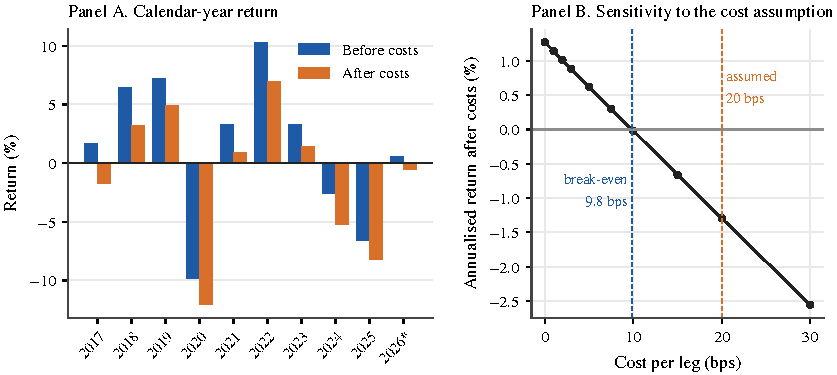
\includegraphics[width=\textwidth]{figures/years_costs.pdf}
\caption{Panel A shows the return in each calendar year before and after costs;
2026 (marked *) is a partial year. Panel B shows the annualised after-cost return
when the same trades are repriced at different costs per leg. Costs are linear in
the rate, so every point is exact, and the value at the assumed \BpsLeg{} basis
points equals the backtest's after-cost return.}
\label{fig:years}
\end{figure}

The single largest loss occurred in the window that began trading on
\WorstWindowStart. Four of the five pairs selected on the 2024
formation period had Kotak Mahindra Bank as a leg, and on \KotakEntry{} all four
were entered on the same day, each short Kotak. The three positions against
public-sector banks, Bank of Baroda, Canara Bank and Punjab National Bank, were
stopped out together on \KotakExit{} for about \rupee\KotakEach{} each, and the
position against Federal Bank on \KotakFedExit{} for \rupee\KotakFedLoss. Together
the four lost \rupee\KotakSameDayLoss{} before costs, about as much as the strategy's
entire gross profit of \rupee\TotalGross{} over nine and a half years. The four
positions were, in effect, a single exposure to Kotak relative to other banks. The
selection rule places no limit on how many selected pairs share a stock, and in
\NConcentrated{} of the \NWindows{} windows one bank was a leg of three or more
selected pairs.

\subsection{Transaction costs}

The signals do not depend on costs, so the same \NTrades{} trades can be repriced at
any cost level (Figure~\ref{fig:years}, Panel B). The break-even follows from the
trade statistics: the mean trade earned \MeanGrossBps{} basis points of notional
before costs, and a round trip costs $2c$ basis points at $c$ basis points per leg,
so $c \approx \BreakEvenSimple$; on the compounded daily series the break-even is
\BreakEven{} basis points per leg. That is about half the assumed cost and within
the range of institutional execution in large Indian banks, but below typical retail
costs. Even at zero cost the strategy would return \RetG{} a year, below the
risk-free rate.

\subsection{Market exposure}

Regressing the strategy's daily after-cost return on the Nifty 50 gives a beta of
\Beta{} and a correlation of \CorrMkt; the market explains \RsqMkt\% of the
strategy's daily variance. A 1\% move in the index is associated with a move of
about \BetaMove\% in the strategy. The long-short construction removed market
exposure as intended, and what remains is a bet on relative price movements between
banks.

% ======================================================================
\section{Discussion}\label{sec:discussion}

The central result concerns persistence. The formation test selects pairs whose
spreads revert at a measurable speed, and when those spreads converged in the
trading period they did so, on average, at almost exactly that speed. But more than
half of the trades were stopped out after the spread widened further, and neither
the formation $p$-value nor repeated selection predicted which. Passing a cointegration test over one year is
evidence that a relationship held over that year; in this sample it was weak
evidence that the relationship would hold over the next six months.

The gross return is consistent with zero. Lower costs would raise the after-cost
return towards the before-cost return, but not above the risk-free rate. This fits
the decline in the profitability of pairs trading reported by \citet{do2010}, and it
suggests that, among the most liquid Indian banks, relationships stable enough to
trade are either rare or already traded.

Concentration produced the largest loss. A limit on the number of selected pairs
that may share a stock would have turned four correlated positions into two, and is
the simplest change likely to reduce the strategy's worst outcomes. The market
neutrality of the construction, by contrast, worked exactly as intended.

% ======================================================================
\section{Limitations}\label{sec:limits}

\begin{itemize}
\item \textit{One sector and one market.} All eleven stocks are Indian banks, and the
  results need not extend to other sectors or markets.
\item \textit{Financing.} No interest is credited on collateral, which would raise
  both return series and make the Sharpe ratio less negative without changing the
  trade-level results. Holding a short equity position in India for more than a day
  requires stock lending or single-stock futures, whose basis and roll costs are not
  modelled.
\item \textit{Costs and execution.} The cost of \BpsLeg{} basis points per leg does
  not vary with volatility or trade size and is probably too low on the days when
  spreads widen sharply, which are the days stops are triggered. All trades are
  executed at closing prices.
\item \textit{Parameters.} The thresholds, the \MaxHold-day limit and the twelve-month
  formation period are conventional values. Testing alternatives properly would
  require a further holdout period.
\item \textit{Survivorship.} The universe consists of banks listed in 2026. Banks
  merged during the sample, such as those absorbed in the 2020 public-sector
  mergers, were never candidates.
\item \textit{Sample sizes.} Several comparisons rest on 60 to 130 trades per group and
  should be read with that in mind.
\end{itemize}

% ======================================================================
\section{Conclusion}\label{sec:conclusion}

A cointegration-based pairs strategy on Indian bank stocks, with every parameter
fixed before it is used, is market-neutral but does not earn a return
distinguishable from zero before costs, and it loses money after them. The reason
is visible in the trades: relationships that passed a cointegration test over twelve
months broke down within weeks more often than they converged, and the strength of
the test statistic did not identify which would hold. The most valuable extensions
address that directly: re-testing cointegration on a rolling window during the
trading period and closing a pair when the test fails, limiting how many selected
pairs may share a stock, estimating the hedge ratio with a Kalman filter, and using
the procedure of \citet{johansen1988} for baskets of more than two stocks.

% ======================================================================
\section*{Use of AI tools}

The research question, the design of the study, the trading rules and tests, and
the interpretation of the results are my own. I used Claude Code, Anthropic's AI
coding assistant, in two supporting roles. The first was as a tutor. When the work
reached an idea I had not used before, such as why a convergence trade needs
cointegration rather than correlation, I asked it to explain the idea and then
checked the explanation against the data before relying on it. The second was implementation: at my direction it wrote parts of the code,
including the plotting code and the script that generates this paper's numbers,
tables and figures, and it helped me draft and edit the text. Working this way also
taught me how to use an AI assistant well, by specifying a task precisely, asking
for the reasoning behind a suggestion and not only the code, and verifying every
output. I reviewed everything it produced and take full responsibility for the
content.

\section*{Data and code availability}

Code, tests and results are available in the project repository,
\weburl{https://github.com/arjunprashanth6129/}{pairs-trading-backtester}. Running the
pipeline regenerates every result from prices it downloads and caches on the first
run, and \code{python paper/make\_assets.py} regenerates every number, table and
figure in this paper from the committed results.

\bibliographystyle{chicago}
\bibliography{references}

% ======================================================================
\appendix
\section{Correction of an entry-rule error}\label{app:fix}

The first complete run of the backtest reported \OldTrades{} trades and an after-cost
return of \OldNet{} a year. A breakdown by exit type showed \OldStops{} stop-outs with
a median holding period of one day. The entry rule had opened a position whenever
$|z_t| \ge \EntryZ$ without checking whether $|z_t|$ also exceeded the stop level. When
a spread moved beyond the stop, the strategy entered, was stopped out the next day
and entered again, for as long as the spread stayed beyond the stop, paying four legs
of cost on each cycle.

\begin{table}[h]
\centering
\caption{The backtest before and after the correction}
\label{tab:fix}
\small
\begin{tabular}{@{}lrr@{}}
\toprule
 & Before correction & After correction \\
\midrule
Round trips & 1,008 & 242 \\
Entered with $|z| \ge 4$ already & 816 & 0 \\
Stopped out & 892 & 130 \\
Median holding period (days) & 1 & 11 \\
Annualised return before costs (\%) & $+$1.04 & $+$1.27 \\
Annualised return after costs (\%) & $-$9.82 & $-$1.29 \\
Maximum drawdown after costs (\%) & 62.16 & 20.17 \\
Break-even cost per leg (bps) & 1.9 & 9.8 \\
\bottomrule
\end{tabular}

\begin{tablenote}
The ``before'' column is computed from the results committed at revision
\code{00591ed}, the last revision before the correction; the ``after'' column is the
current backtest.
\end{tablenote}
\end{table}

The correction adds one condition, no entry while $|z_t| \ge \StopZ$, and two tests
cover it. A position may be opened once the spread returns inside the stop level.
The error changed the after-cost return by \FixNetChange{} percentage points a year
and the before-cost return by only \FixGrossChange{}. Because its effect appeared
almost entirely as cost, the first run looked like a strategy with a gross edge that
could not cover its costs. The decomposition by exit type showed that this reading
was wrong, and it is the reason the decomposition appears in the main results.

\end{document}
